\documentclass[../main.tex]{subfiles}

\begin{document}
    Im Folgenden soll der Einfluss von paramagnetischen Salzen auf die longitudinale Relaxationszeit $T_{1}$ und die transversale Relaxationszeit $T_{2}$ untersucht werden. Paramagnetische Salze besitzen Ionen mit freien, ungepaarten Elektronen, die eine positive magnetische Suszeptibilität $X > 0$ besitzen. Sie haben also einen verstärkenden Effekt auf das umgebende Magnetfeld und somit insbesondere auf das im Verlauf der Messung angelegte Polarisationsfeld. In der Medizin wird diese Eigenschaft unter anderem angewendet, um bestimmte Stoffe im Körper von anderen zu unterscheiden. So kann nach einem Schlaganfall, Blut im Gehirn detektiert werden, da ein verabreichtes Kontrastmittel nur im Blut vorhanden ist. Der physikalische Hintergrund liegt bei den beiden Relaxationszeiten, die beide durch das stärkere Magnetfeld kürzer, also unterdrückt werden. Dabei sorgt die Abnahme der longitudinalen Relaxationszeit $T_{1}$ der Spin-Gitter-Relaxation für eine Verstärkung des zugrunde liegenden Signals. Man spricht daher von einem positiven Kontrast. Die Reduzierung der transversalen Spin-Spin-Relaxationszeit $T_{2}$ bewirkt hingegen die Abschwächung des Signals. Man spricht hier deshalb vom negativen Kontrast. Der Einfluss von $T_{1}$ ist in der Regelstärker als der von $T_{2}$. Erst bei Polarisationsdauern, bei denen sich $T_{1}$ in der Sättigung befindet zeigt der Einfluss $T_{2}$ seine Wirkung. Das wird im nachfolgenden Versuchsteil deutlich, wenn zwei Röhren mit verschiedenen Ionenkonzentrationen angeregt werden. Ziel dieses Teils ist es die Relaxivitäten $r_{1}$ und $r_{2}$ zu bestimmen. Sie sind ein Maß für die Güte des Kontrastmittels. \\
    Zur Durchführung wurden insgesamt vier Flaschen mit einer Ionenkonzentration von \SI{25}{\micro \mol \per \litre}, \SI{50}{\micro \mol \per \litre}, \SI{100}{\micro \mol \per \litre} und \SI{200}{\micro \mol \per \litre} verwendet. Bei den Ionen handelt es sich um Mangan (\ce{Mn^2+}) und Chlor (\ce{Cl^2-}) aus dem im Wasser gelösten \ce{MnCl2}. Zunächst wurde die $T_{1}$-Relaxationszeit (longitudinal) für die verschiedenen Proben ermittelt. Diese sind in Abb. \ref{fig:Relaxation_T1} dargestelt.
    \begin{figure}[h!]
        \centering
        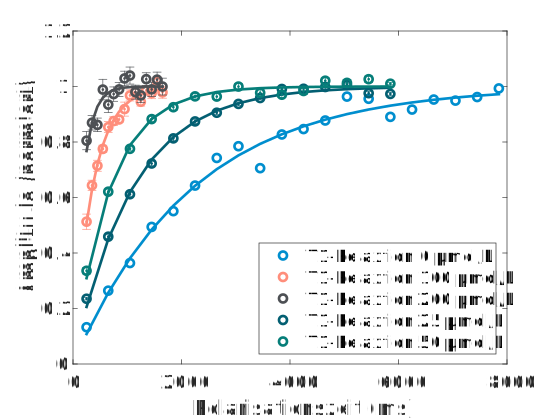
\includegraphics[width=\textwidth]{Bilddateien/11/T1/Part_11_Fig_6}
        \caption{$T_{1}$-Relaxationszeit in Abhängigkeit der Polarisationszeit und der Ionenkonzentration in der Probe. An den Messpunkten ist eine Kurvenanpassung nach Gl. \ref{eq:T1_Relaxation} angelegt worden.}
        \label{fig:Relaxation_T1}
    \end{figure}
    Zum Vergleich wird die Messung für $T_{1}$ aus dem vorherigen Versuchsteil, nach der Kalibrierung mit in diesem Graphen dargestellt. Dort wurde eine Flasche ohne gelöste Ionen gemessen. Die Konzentration betrug also \SI{0}{\micro \mol \per \litre}. An die Messdaten wird die Exponentialfunktion aus Gl. \ref{eq:T1_Relaxation} angepasst.
    \begin{align} \label{eq:T1_Relaxation}
        A(t) = A_{0} \cdot \left[1 - \exp\left( \frac{t}{T_{1}}\right) \right]
    \end{align}
    Es ist deutlich erkennbar, dass $T_{1}$ mit steigender Ionenkonzentration abnimmt und das Signal viel früher sättigt. Ebenfalls ist zu erkennen, dass das Signal bei größerer Ionenkonzentration insgesamt instabiler wird und die Unsicherheit zunimmt. 
    \begin{figure}[h!]
        \centering
        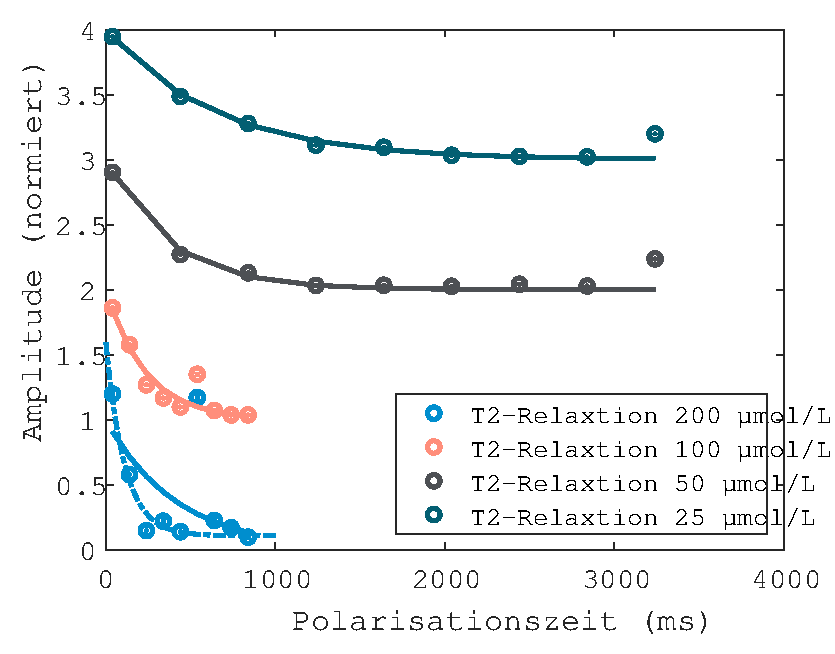
\includegraphics[width=\textwidth]{Bilddateien/11/T2/Part_11_Fig_5}
        \caption{$T_{2}$-Relaxationszeit in Abhängigkeit der Polarisationszeit und der Ionenkonzentration in der Probe. Zur besseren Sichtbarkeit wurden die normierten Amplituden auf der y-Achse um jeweils 1 verschoben. An den Messpunkten ist eine Kurvenanpassung nach Gl. \ref{eq:T2_Relaxation} angelegt worden. Der Fit für \SI{200}{\micro \mol \per \litre} wurde manuell wiederholt (gestrichelte Linie).}
        \label{fig:Relaxation_T2}
    \end{figure}
    Für $T_{2}$ wird die im Programm integrierte Methode zur Messung von $T_{2}$ verwendet. In Abb. \ref{fig:Relaxation_T2} ist die Abhängigkeit der transversalen $T_{2}$-Relaxationszeit aufgetragen. Die Werte der Amplituden sind normiert und jede Messung ist auf der y-Achse um den Wert 1 zur vorherigen verschoben. Dies soll für eine bessere Darstellung der Daten sorgen und hat keine weitere Bedeutung. 
    \begin{align} \label{eq:T2_Relaxation}
        A(t) = A_{0} \cdot \exp\left( \frac{t}{T_{2}}\right)
    \end{align}
    An die Messdaten ist die Gl. \ref{eq:T2_Relaxation} angepasst. Aus den Messdaten lässt sich der vermutete Zusammenhang ableiten, dass die $T_{2}$-Relaxationszeit für höhere Ionenkonzentrationen abnimmt. Bei der Messung für \SI{200}{\micro \mol \per \litre} sind die Daten leider so verrauscht, dass der Fit aus dem Messprogramm nicht zur Erwartung passt. Deshalb wurde dieser Fit in der Auswertung wiederholt. Dabei wurde der ausreißende Punkt bei $t_{pol} = \SI{550}{\milli \second}$ nicht berücksichtigt. Auffallend ist, dass dieser Messpunkt auch bei der Messung mit der Konzentration von \SI{100}{\micro \mol \per \litre} ausreißt, wenn auch bei weitem nicht so stark wie in der \SI{100}{\micro \mol \per \litre}-Messung. 
    \begin{table}[h!]
        \centering
        \begin{tabular}{l|llll}
        Ionenkonzentration                  & $T_{1}$                     & $T_{2}$                    & $u(T_{1})$                & $u(T_{2})$                 \\ \hline
        $\SI{25}{\micro \mol \per \litre}$  & $\SI{1090}{\milli \second}$ & $\SI{640}{\milli \second}$  & $\SI{30}{\milli \second}$ & $\SI{90}{\milli \second}$  \\
        $\SI{50}{\micro \mol \per \litre}$  & $\SI{680}{\milli \second}$  & $\SI{419}{\milli \second}$ & $\SI{20}{\milli \second}$ & $\SI{100}{\milli \second}$ \\
        $\SI{100}{\micro \mol \per \litre}$ & $\SI{350}{\milli \second}$  & $\SI{230}{\milli \second}$ & $\SI{10}{\milli \second}$ & $\SI{50}{\milli \second}$  \\
        $\SI{200}{\micro \mol \per \litre}$ & $\SI{170}{\milli \second}$  & $\SI{111}{\milli \second}$ & $\SI{10}{\milli \second}$ & $\SI{186}{\milli \second}$
        \end{tabular}
        \caption{Ermittelte Relaxationszeiten $T_{1}$ und $T_{2}$ für die verschiedenen Ionenkonzentrationen.}
        \label{tab:RelaxT}
    \end{table}
    Die aus den Fits ermittelten Werte für $T_{1}$ und $T_{2}$ sind in Tab. \ref{tab:RelaxT} aufgetragen. Für die Relaxivität $r_{i}$ gilt der Zusammenhang
    \begin{align} \label{eq:Relaxivität}
        \frac{1}{T_{i}([X])} = r_{i} \cdot [X] + \frac{1}{T_{i}(0)}.
    \end{align}
    Dabei ist $[X]$ die Ionenkonzentration und $r_{i}$ die Relaxivität. Um die Relaxivität zu ermitteln, wird der Kehrwert der Relaxation über der Ionenkonzentration aufgetragen und mittels linearer Anpassung nach Gl. \ref{eq:Relaxivität} bestimmt. Das ist in Abb. \ref{fig:Relaxivität} gezeigt.
    \begin{figure}[h!]
        \centering
        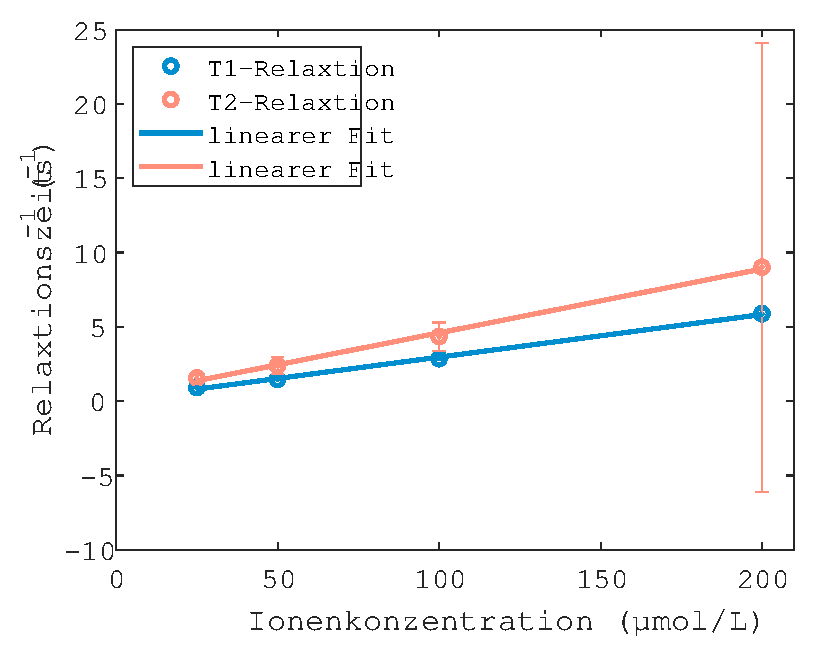
\includegraphics[width=\textwidth]{Bilddateien/11/R12/Part_11_T1T2_Fig_1}
        \caption{Kehrwerte von den Relaxationszeiten $T_{1}$ und $T_{2}$ aufgetragen über der Ionenkonzentration. Die Steigung der beiden Anpassungsgeraden entspricht der Relaxivität. Es zeigt sich: $r_{1} = \SI{0,029 +- 0,028}{\litre \per \micro \mol \second}$ und $r_{2} = \SI{0,043 +- 0,038}{\litre \per \micro \mol \second}$}
        \label{fig:Relaxivität}
    \end{figure}    
    Bei Betrachtung der Graphen fällt auf, dass die Unsicherheiten bei höheren Konzentrationen sehr groß werden. Insbesondere bei $T_{2}$ ist das deutlich zu erkennen. Eine Erklärung dafür ist, dass sich die Unsicherheiten nach
    \begin{align}
        u(\frac{1}{T}) = \sqrt{\left(\frac{1}{T^{2}} \cdot u(T) \right)^{2}}
    \end{align} berechnen.
    Das sorgt für ein starkes Ansteigen bei kleinen Werten von $T$ bei denen die Unsicherheiten $u(T)$ ebenfalls etwas größer sind. Für die Relaxivitäten ergibt sich
    \begin{align*}
        r_{1} = \SI{0,029 +- 0,028}{\litre \per \micro \mol \second} \\
        r_{2} = \SI{0,043 +- 0,038}{\litre \per \micro \mol \second}
    \end{align*}.
    Die Unsicherheiten der Werte bewegen sich im Bereich des ermittelten Wertes, was bei der Größe der Unsicherheiten von den Kehrwerten der Relaxationszeiten nicht ungewöhnlich erscheint. 
\end{document}